\section{The effect of switching types}
\label{section:switch}
Segregation is a phenomenon taking many different forms. Rather than  limiting the scope to racial segregation, we decided to broaden our view. 
For example, one might delve into the segregation in studies with respect to friendship. 
In this case, for any person \(k\), the neighbours of \(k\) represent \(k\)'s friends or the persons with whom \(k\) spends most of his time.
In this case, \(k\)'s type, can represent either the classes he is currently taking, or the kind of sports person \(k\) is doing, or more realistically, \(k\)'s political beliefs.
In any of these cases, the type of \(k\) is not necessarily set indefinitely.\\
In these cases, the type of \(k\) might switch, depending on the types of his friends. This is a sociological process known as conformation and plays a major role in the everyday behaviour of people.\\


This gives rise to a new modification of the model.
For any person \(k\), before moving to a new location, \(k\) has a catagorical probability with to switch to a different type, where 
\[\mathbb{P}(\text{NewType}(k)=t) = \begin{cases} 
 \frac{\#\text{Neighbours of type }t}{\text{Total number of neighbours}}	&\mbox{if } \text{total number of neighbours}>0 \\ 
\mathbbm{1}_{\{t=\text{Type}(k)\}}   &\mbox{if } \text{total number of neighbours}=0
\end{cases}\]
Note that this is well defined, since if total number of neighbours \(> 0\), we have \( \mathbb{P}(\text{NewType}(k)=t) \geq 0\) and \(\sum_{i=0}^{\text{types}}\mathbb{P}(\text{NewType}(k)=t)=1\). An example of how this may effect the equilibrium, is illustrated below:

\begin{figure}[H]
	\centering
    \begin{subfigure}{0.45\textwidth}
        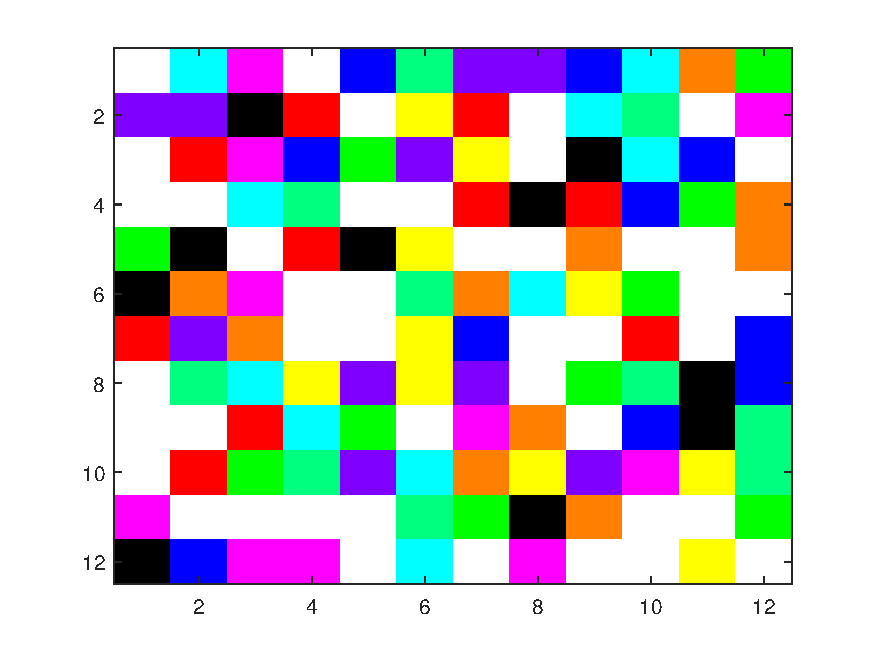
\includegraphics[width=\textwidth]{Voorbeeld12_12_begin}
        \caption{Situation before segregation}
        \label{fig:wis12b}
    \end{subfigure}\hspace{0cm}
    ~ 
    \begin{subfigure}{0.45\textwidth}
        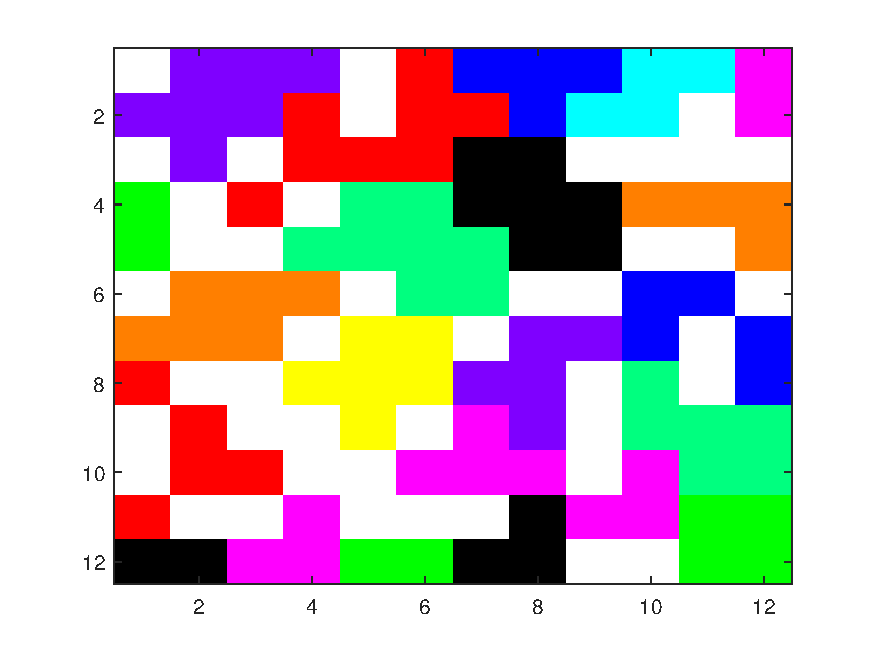
\includegraphics[width=\textwidth]{Voorbeeld12_12_eind}
        \caption{Situation after segregation}
        \label{fig:wis12a}
    \end{subfigure}
    ~ 
    \caption{An illustration of the effect of switching types on the \(12 \times 12\) Board}
    \label{fig:wissel 12}
\end{figure}

A crucial difference between equilibrium with and without switching, is that if switching is allowed, the concentration of the types may differ between the starting board and the equilibrium status. 
This can be seen in figure \ref{fig:wissel 12} as the number of people of the green type decreased from 10 to 8, the yellow type even decreased from 10 to 6. 
As a matter of fact, allowing switching might lead to the extinction of several types. 

This is not generally the case for lower bounds on the happiness rule, but if the happiness rule is increased, several types might cease to exist. Despite this being quite interesting, the extinction of types is not included in this report.
What will be studied in this report, is the effect of switching, on the given research questions. In other words, how will the results discussed in this report, vary when switching types is allowed. 
\newpage

\subsection{Average number of generations until equilibrium}\label{subsec:avegensw}
First, the effect of switching on the average number of generations until equilibrium will be discussed. 
From figure \ref{fig:avegen}, we deduced that on average, a board reaches equilibrium in only a few generations. This however decreases even more drastically when switching goes in effect:

\begin{figure}[H]
	\centering
    \begin{subfigure}{0.9\textwidth}
        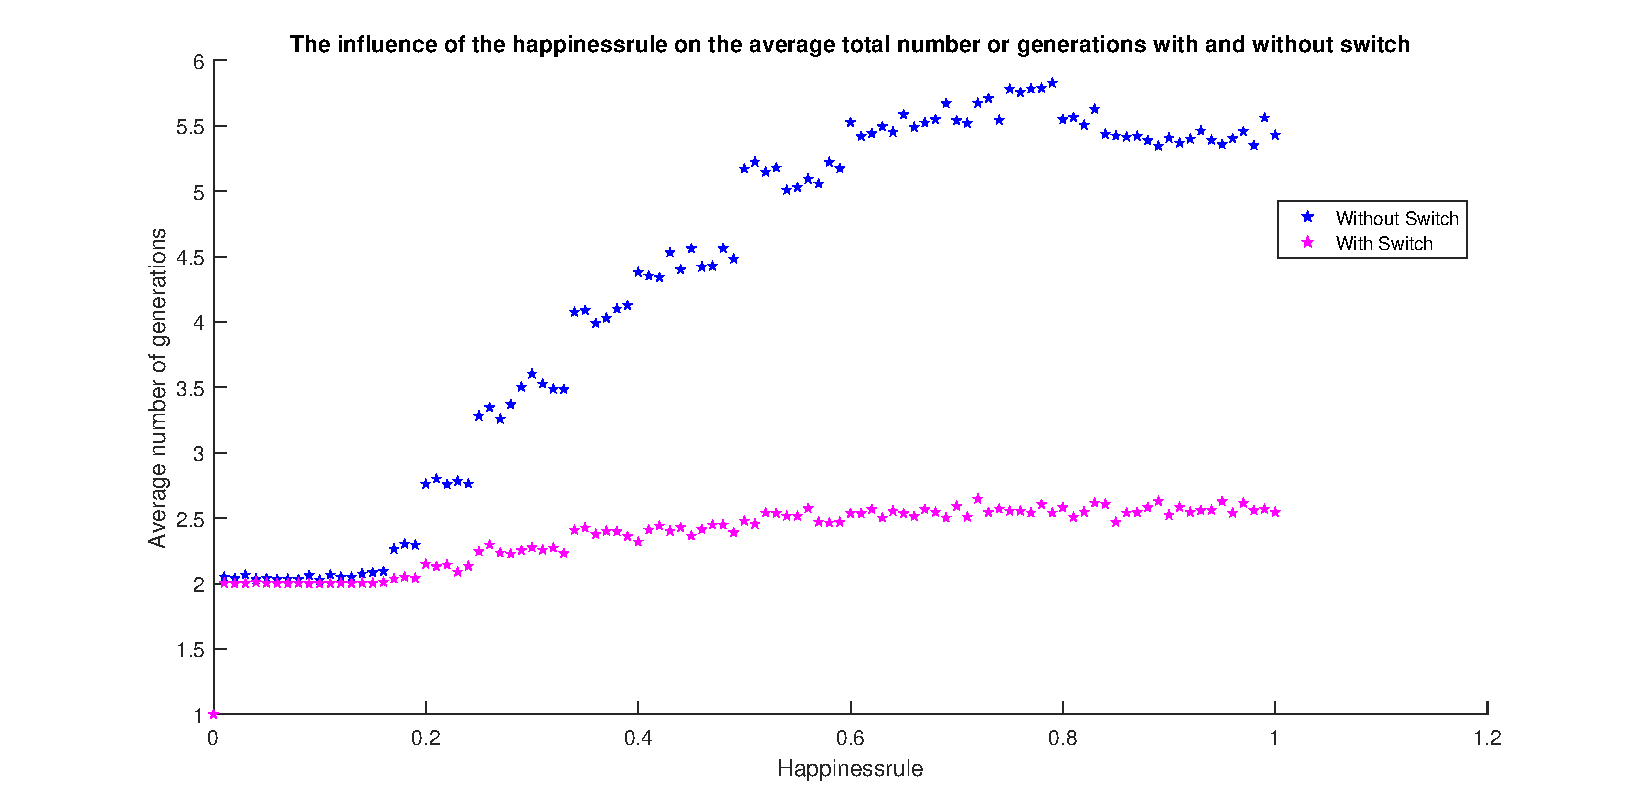
\includegraphics[width=\textwidth]{happinessrule-totaantgenwithswitchorwithoutswitch}
    \end{subfigure}
    \caption{Number of generations until equilibrium on an 8x8 board with standard setting, with and without type switching}
    \label{fig:AantGenS}
\end{figure}

In figure \ref{fig:AantGenS}, we see a comparison of the average number of generations for with and without type switching. 
Clearly, when type switching is applied, it takes much less generations to reach the equilibrium. 
This is expected, since the probability of becoming the same type as the neighbours is more favored in this model, which results in an increase of happiness. 
Or, in a sociological view, the person is willing to adapt to the environment rather than moving on.\\

From figure \ref{fig:AantGenS}, we observed that the average number of generations to reach equilibrium is nearly constant for any HR in the interval \((0.6,1)\). 
Just to get an idea whether this statement is justified, we selected three HR's, namely 0.6, 0.8 and 1 and performed the two sample t-test(for more description about this test, see section Model and Statistical Methods) in Matlab. Because the histograms show that the data might follow an asymmetric distribution and this t-test requires the difference of the means to be normally distributed, we chose a sample size of 50000 to ensure normality through the Central Limit Theorem.\\
\\
The sample means are shown in Table 3:
\begin{table}[htp]
\centering
\caption{Sample means of number of generations to reach equilibrium simulated with HR 0.6, 0.8 and 1, with 50000 sample size for each HR.}
\begin{tabular}{|l|l|l|l|}
\hline
 HR&0.6&0.8&1 \\ \hline
 Sample Mean&2.5213&2.5616&2.5711  \\ \hline 
\end{tabular}
\end{table}
\\
We applied the t-test twice. First time comparing the mean of HR 0.6 and 0.8. Second time for comparing the mean of 0.8 and 1. The first test rejected the null-hypothesis, the second did not. So with 95\% confidence level, we may conclude that the average generations are unequal for HR 0.6 vs 0.8, but equal for HR 0.8 vs 1.\\
\newpage
Similar to section 4, in order to get an idea about the distribution of the random variable of $Y_{j,s}$(referring to the notation in section 4, with s meaning type switching), we plotted again histograms for HR $\frac{1}{4}$, $\frac{1}{3}$, $\frac{1}{2}$ and $1$ in figure \ref{fig:histogramSw}.

\begin{figure}[H]
    \centering
    \begin{subfigure}{0.45\textwidth}
        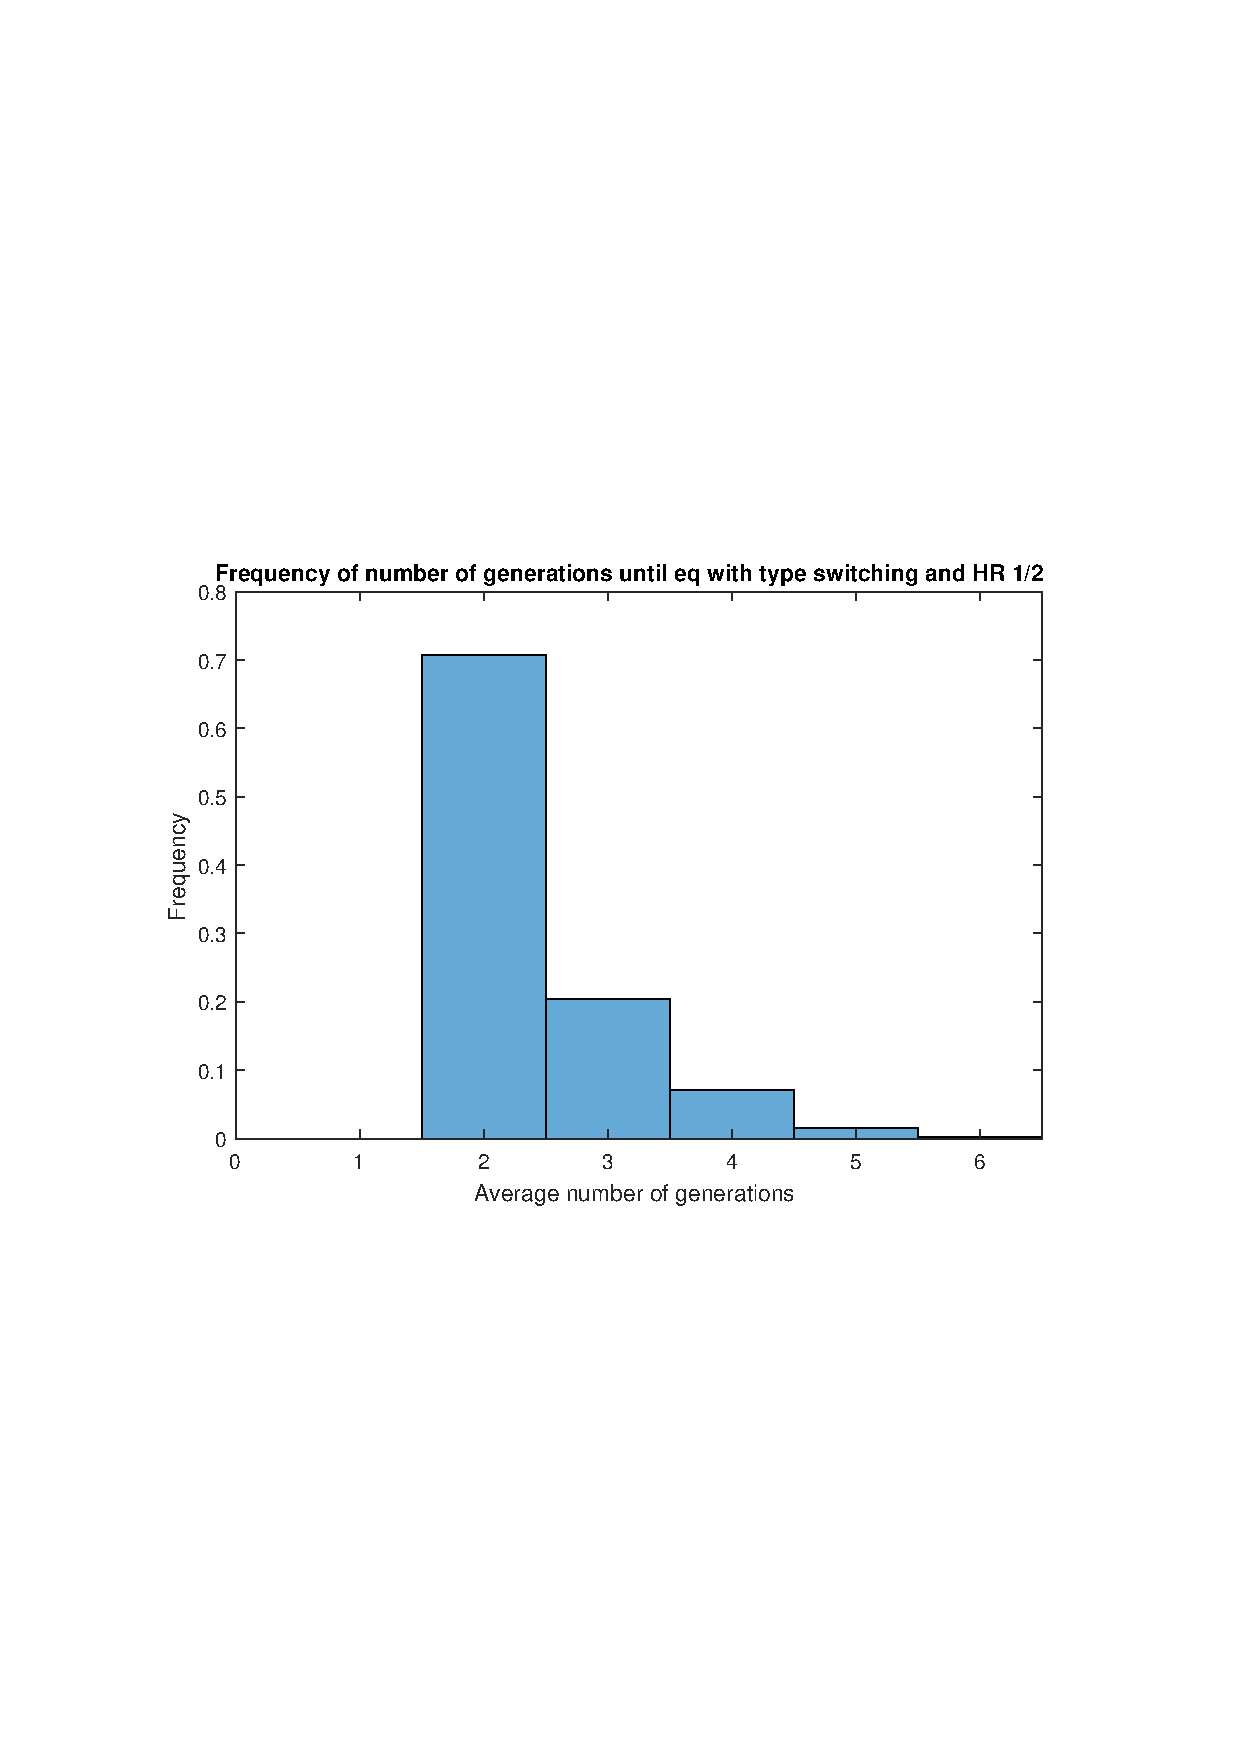
\includegraphics[width=\textwidth]{AantGen1.pdf}
        \caption{5000 simulations of number of generations until equilibrium with HR $\frac{1}{4}$ with switch}
        \label{hists hap 1/4}
    \end{subfigure}
	~
    \begin{subfigure}{0.45\textwidth}
        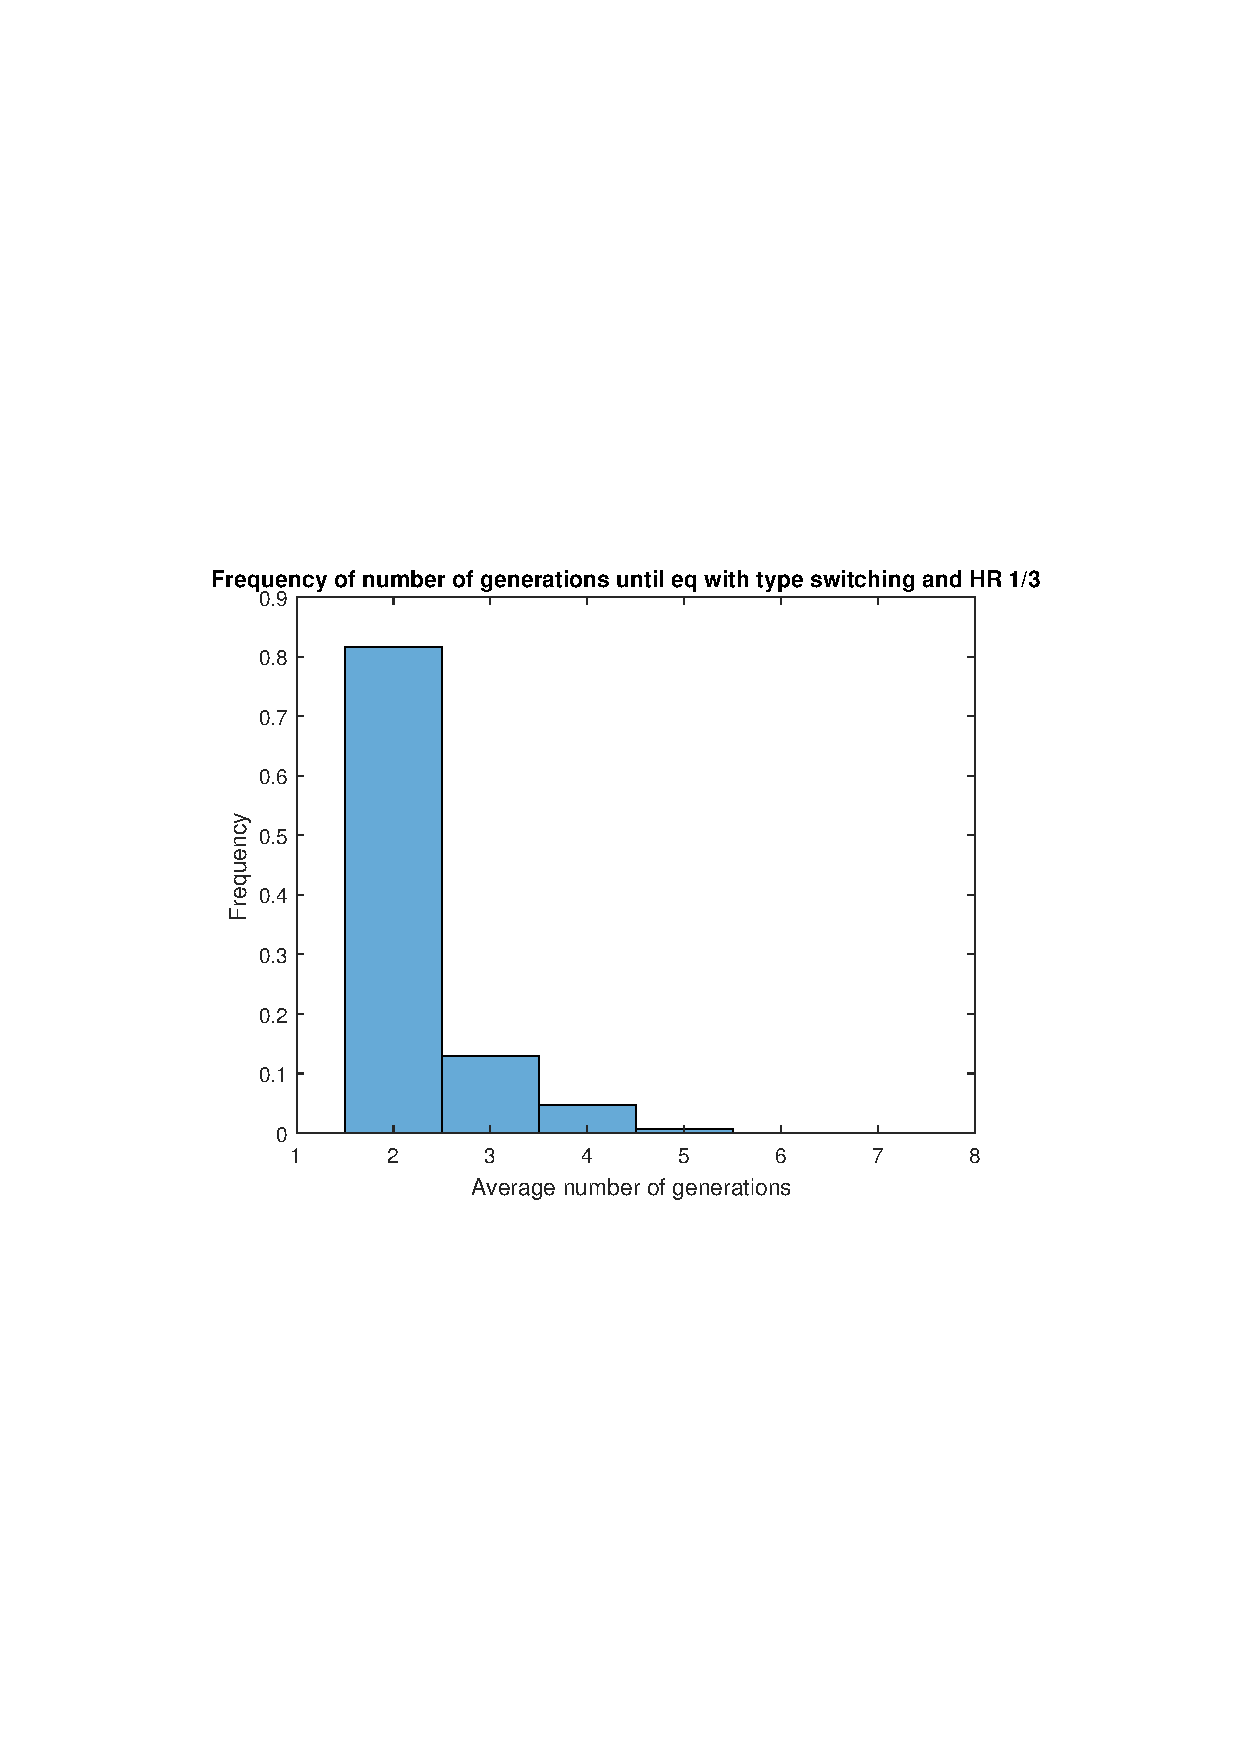
\includegraphics[width=\textwidth]{AantGen2.pdf}
        \caption{5000 simulations of number of generations until equilibrium with HR $\frac{1}{3}$ with switch}
        \label{hists hap 1/3}
    \end{subfigure}
	~
    \begin{subfigure}{0.45\textwidth}
        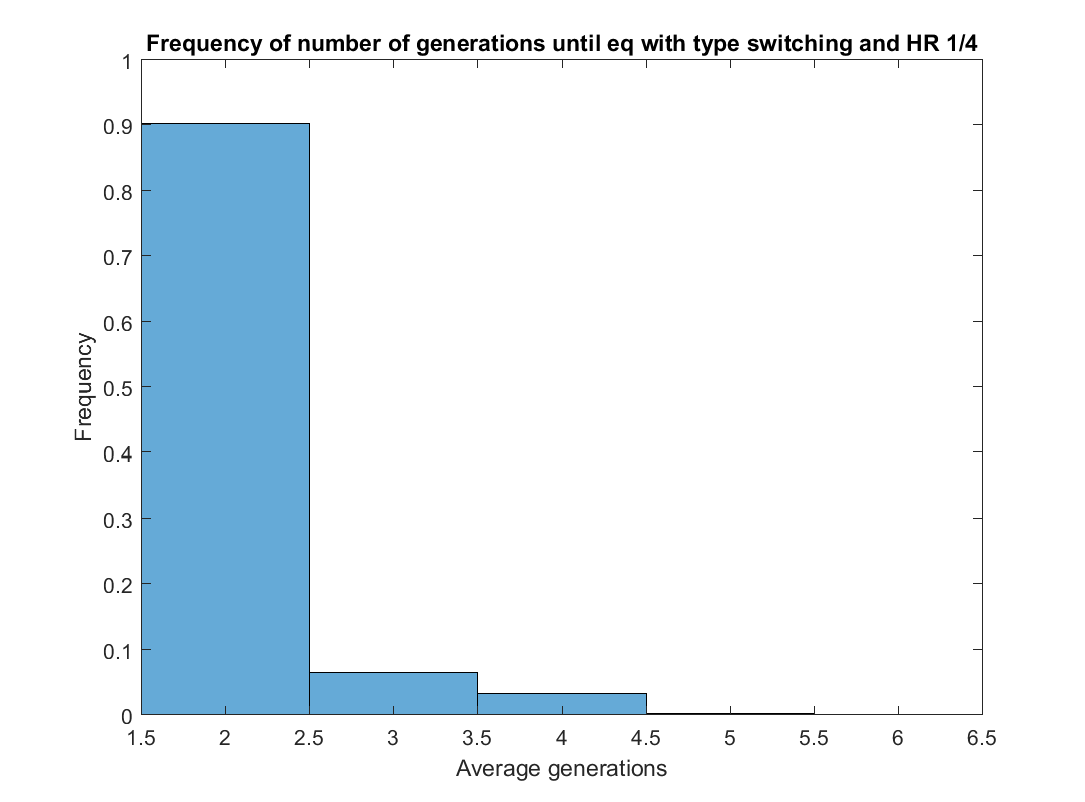
\includegraphics[width=\textwidth]{AantGen3.pdf}
        \caption{5000 simulations of number of generations until equilibrium with HR $\frac{1}{2}$ with switch}
        \label{hists hap 1/2}
    \end{subfigure}
    ~
    \begin{subfigure}{0.45\textwidth}
        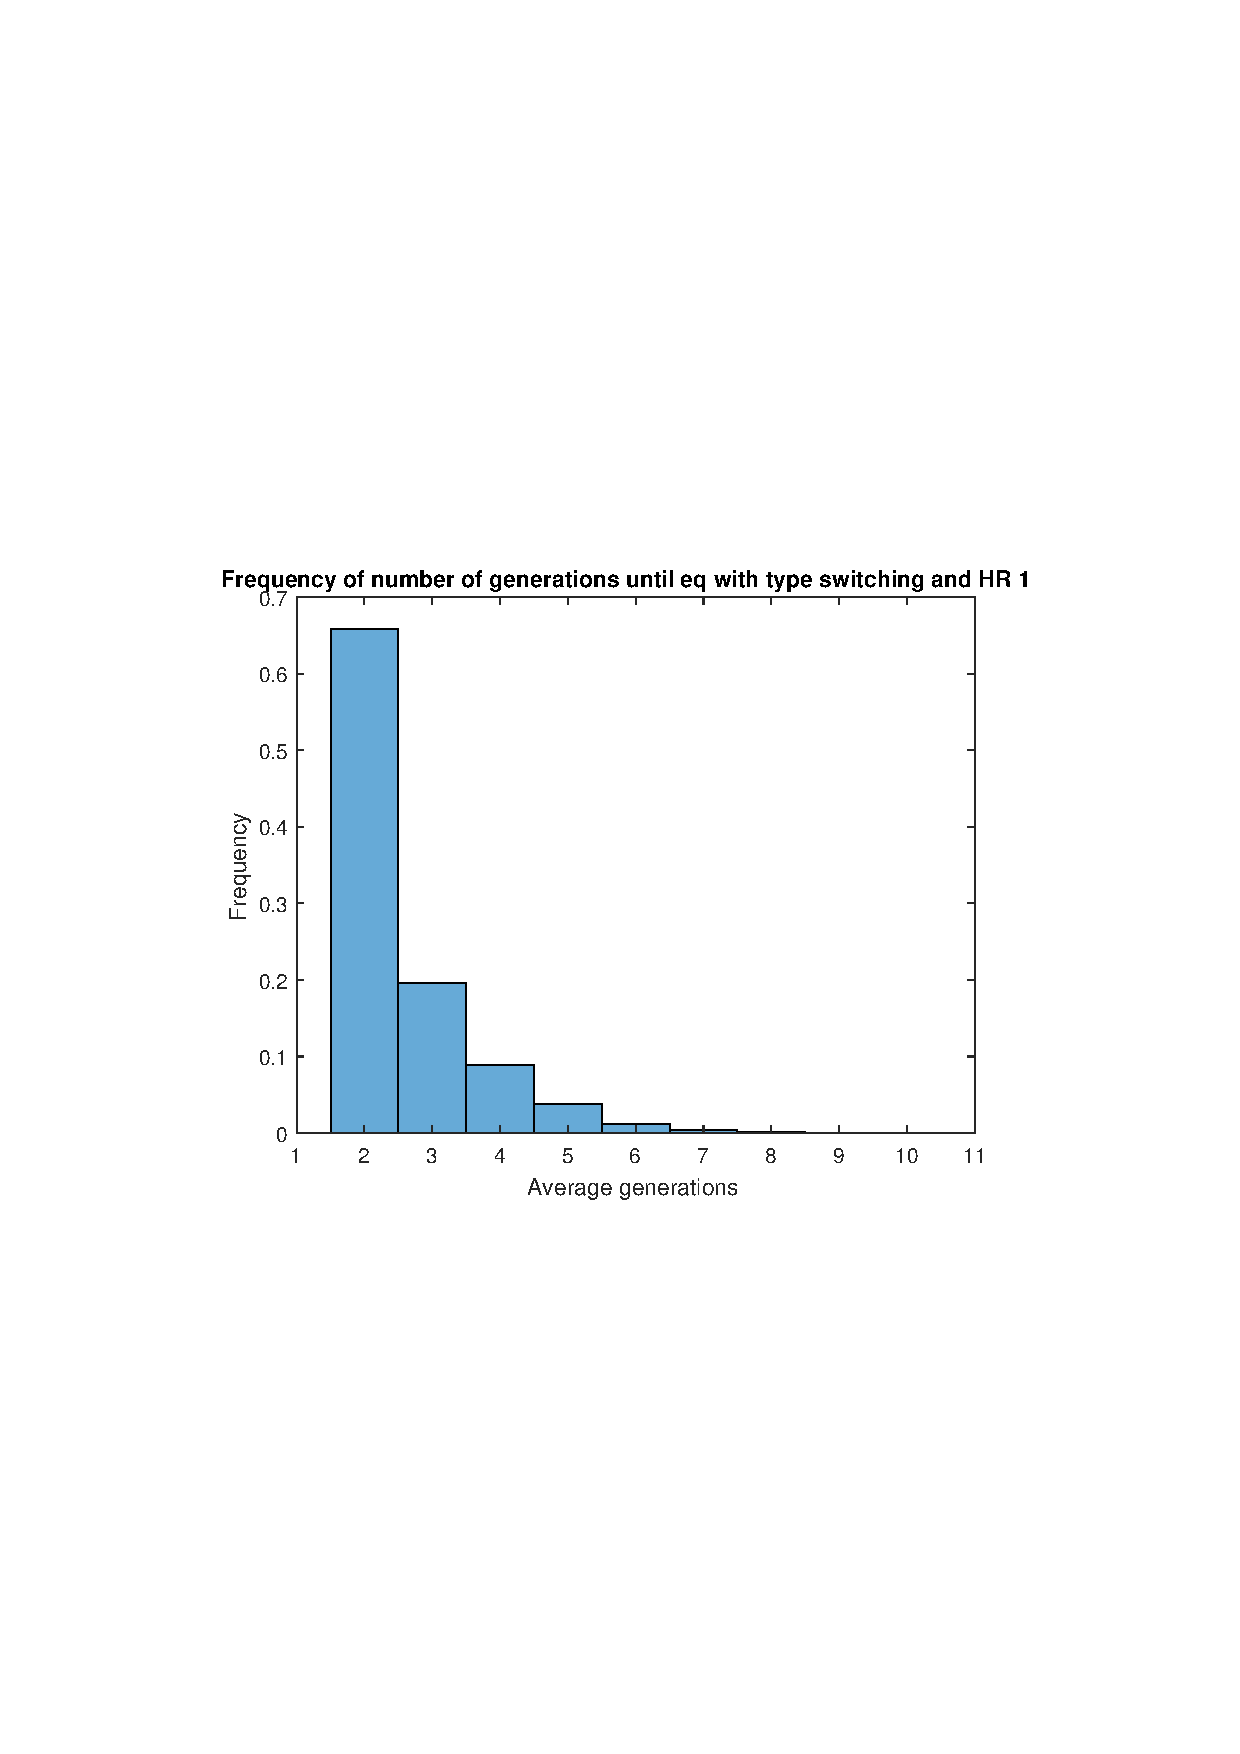
\includegraphics[width=\textwidth]{AantGen4.pdf}
        \caption{5000 simulations of number of generations until equilibrium with HR 1 with switch}
        \label{hists hap 1}
    \end{subfigure}
    \caption{The probability distribution of $Y$ (the number of generations until reaching the equilibrium) is approximated with a histogram of bin size 1. 
    For each HR ($\frac{1}{4}$, $\frac{1}{3}$, $\frac{1}{2}$ and $1$), $5000$ simulations were ran.}
    \label{fig:histogramSw}
\end{figure}

Again, all $Y_{s,j}$'s appear to be following the same distribution just as without switch (section 4). 
The histograms suggest that the $Y_{j,s}$'s might follow a geometrical distribution, which is a Negative Binomial with $r=1$. 
But we could not perform the same statistical analysis as in section 4, because the maximum likelihood estimators for the Negative Binomial could not be calculated through the fitdist or other functions. 
This is due to the fact that the sample means exceeded the sample variance. So from this we could conclude that $Y_{j,s}$'s cannot be geometrically (or NB) distributed.\\

It is much more interesting to compare the distribution of $Y_{j,s}$ with $Y_{j}$. A remarkable observation is that the histograms of $Y_{j,s}$ completely lost it's symmetry compared to the histograms of $Y_j$. 
Apparently, type switching stimulates segregation so well that it only takes 1 generation to reach equilibrium (remark: we always start with 1 generation, so the fastest segregation is reached at the 2nd generation).\\
\\ 
To further examine how type swithcing affects generations until equilirbium, we chose to compare $Y_{1,s}$ with $Y_1$ in a QQ-plot:

\begin{figure}[H]
    \centering
    \begin{subfigure}{0.8\textwidth}
        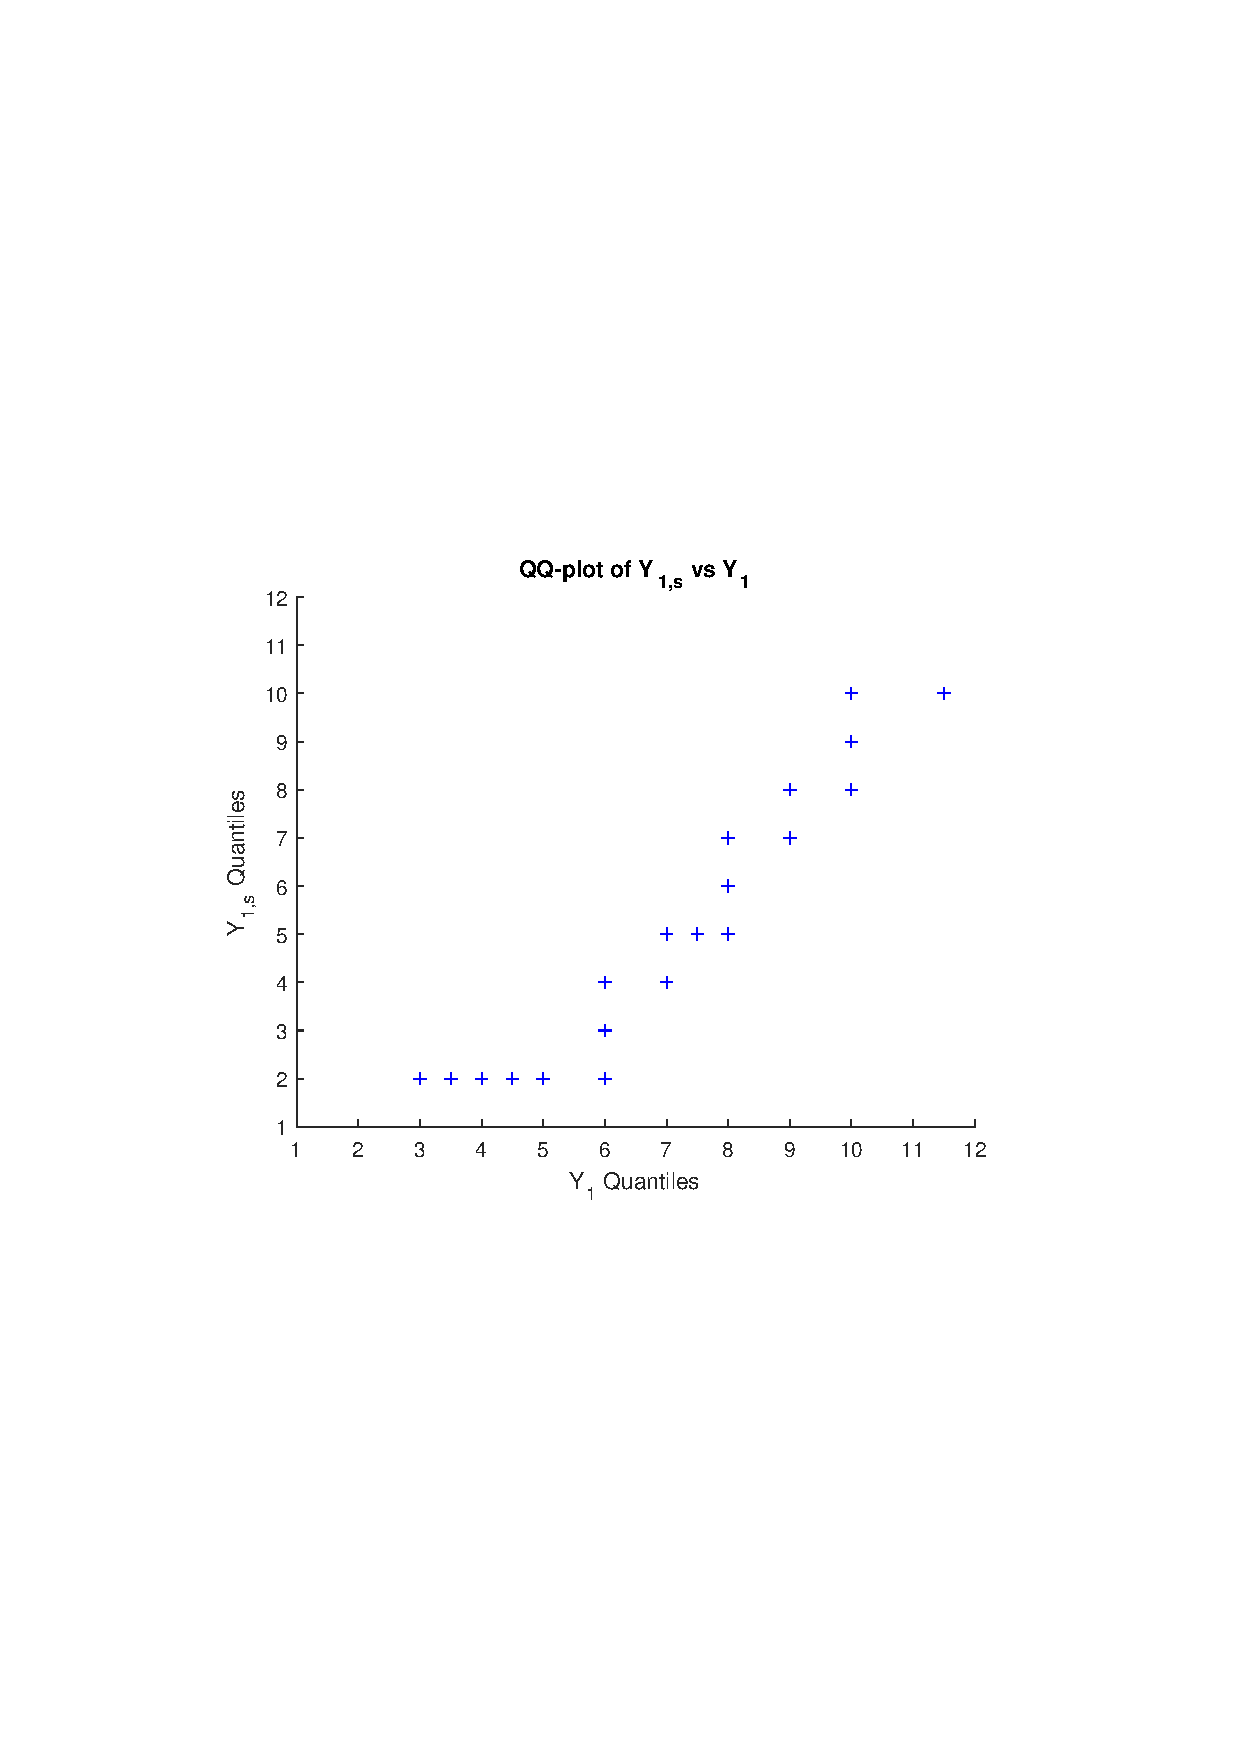
\includegraphics[width=\textwidth]{QQplotY1sw.pdf}
    \end{subfigure}
    \caption{QQ-plot of $Y_{1,s}$ vs $Y_1$}
    \label{fig:QQplotSw}
\end{figure}  

Starting from quantile 3 of $Y_1$, the line is flat, which is expected because the most quantile of $Y_{1,s}$ is concentrated on 2. After the flat line we see a linear pattern, which suggests that the 'tail' part of $Y_{1,s}$ and $Y_1$ are not too differently distributed. This is also seen by comparing the figure \ref{fig:histogramSw} with figure 9.

\subsection{Happiness at equilibrium}

Secondly, we investigate the effect of the ability to switch type on the mean happiness after the equilibrium is reached.
We research this effect for different values of the Happiness Rule like we did in section \ref{sec:meanhappy}.
In this section, we found that the mean happiness at equilibrium increases as the Happiness Rule gets higher.
Intuitively, we expect a higher happiness when individuals can switch type, because the chance to become happier by switching is really big.
This follows directly from the probability distribution we defined earlier in this section.\\

Now, we will make the same graph for the same settings except for switch; we turn it on. 
Then, we can compare these results.
We make this comparisation in figure \ref{fig:meanhappyswitch}.

\begin{figure}[H]
    \centering
    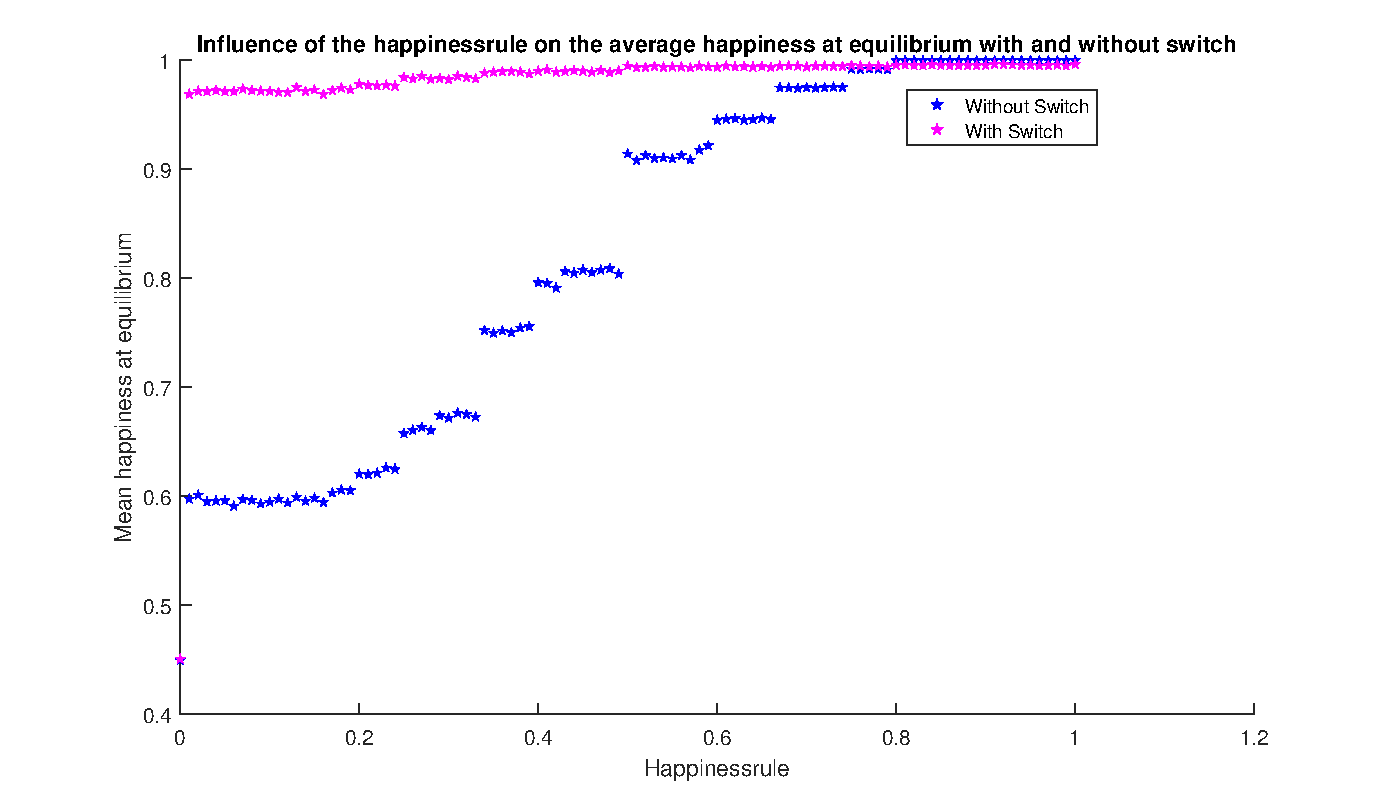
\includegraphics[width=0.8\textwidth]{happinessrule-meanhappiness-switch.pdf}
    \caption{The effect of the ability to switch and the Happiness Rule on the mean happiness at equilibrium}
    \label{fig:meanhappyswitch}
\end{figure}

This is a really nice result.
It seems that switch causes a much higher average happiness in equilibrium, as expected.
However, for Happiness Rules higher than $0.8$, we see that the mean happiness on the board is a little bit lower, if the individuals can change type.
This can maybe be explained by the number of generations.
We already saw that mean number of generations is less if switch is included.
That implies less chances for each individual to get a happiness as high as possible.
Thus, the mean happiness will be lower.
For the lower Happiness Rules, the switch has a much higher influence, because the chance to get a high happiness is significantly higher than keeping a lower happiness.

\subsection{Average segregation time}
The final topic to be discussed in this report, will be the effect of conformation on the (average) segregation time. 
For this purpose, we will compare the results obtained in section \ref{sec:aveseg} with the results if switching were allowed. 
We will only consider the results for the standard board.\\
For any \(p\in [0,100]\). We will consider the time until which \(p\%\) of the population lives in homogenous groups. With a chosen HR of 1, we obtain:

\begin{figure}[H]
    \centering
    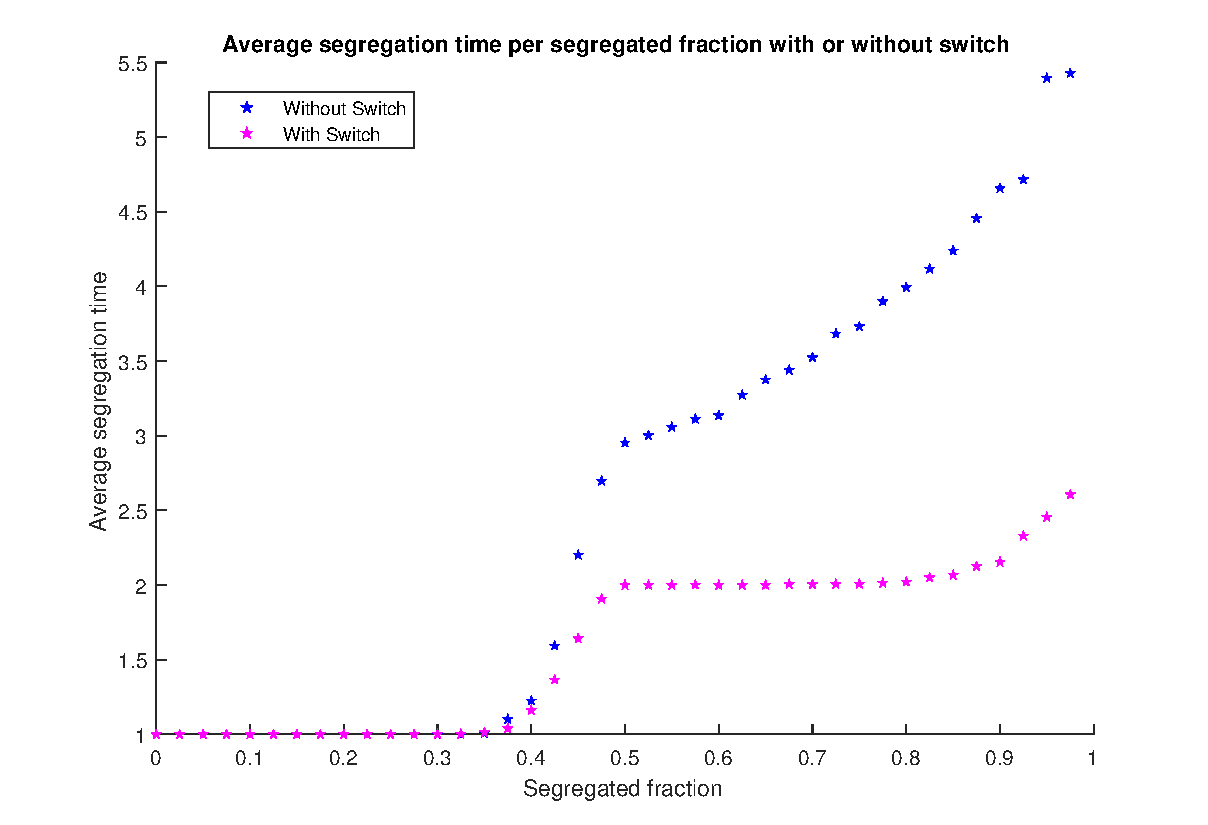
\includegraphics[width=0.8\textwidth]{Avesegsw2}
    \caption{The average segregation as a function of the segregation fraction with switch (pink) and without switch (blue)}
    \label{fig:avesegsw}
\end{figure}

From figure \ref{fig:avesegsw}, the hypothesis that the average segregation time is lower for every fraction, if switching is allowed. 
A less trivial result of conformity, is that the average segregation time is nearly constant between the fractions \(0.5\) and \(0.8\). 
To test whether it is justified to make this claim, we will conduct the \(t\)-test as described in section \ref{subsec:avegensw}. We will test if the segregation time at \(60\%\) and \(80\%\) have the same mean value if 5000 simulations are ran each. 
The \(t\)-test, rejected the null-hypothesis that \(60\%\) segregation and \(80\%\) segregation share the same mean value. When the respective means were 2 and 2.0136. As mentioned in the introduction, a mean of 2 generations implies here, that the board has reached \(60\%\), in at most 1 generation (Every individual has moved or switched type only once at most.)
We conclude that on the standard board with HR 1, segregation at \(p\%\) takes place in less than one generation, for any \(n\leq 0.7\). 
It is interesting to note that both graphs appear constant for any \(q\leq \frac{1}{3}\). 
This can be explained as follows. In both scenarios, the segregated fraction has been reached, by the boards default setup and thus no person will move before segregation has been reached.
Another remarkable similarity between both graphs, is that they tend to grow with the same order between a fraction of 0.3 and 0.5.
